\documentclass[sigconf]{acmart}

\usepackage{booktabs} % For formal tables
\usepackage{subcaption}
\usepackage{multicol}

\acmPrice{15.00}

% The next six lines come directly from the completed rights form.
% You MUST replace them with the lines specific to your accepted work.

\copyrightyear{2019}
\acmYear{2019}
\setcopyright{rightsretained}
\acmConference{CMPM 164}{Fall 2019}{Santa Cruz}
\acmDOI{}
\acmISBN{}

% Use the "authoryear" citation style, and make sure citations are in [square brackets].
\citestyle{acmauthoryear}
\setcitestyle{square}

% A useful command for controlling the number of authors per row.
% The default value of "authorsperrow" is 2.
\settopmatter{authorsperrow=2}

% end of preamble.

\begin{document}

% Title. 
% If your title is long, consider \title[short title]{full title} - "short title" will be used for running heads.
\title{Exploring Chaos Destruction with Niagara Particle System in Unreal Engine 4}

% Authors.
\author{Yanwen Xu}
\affiliation{%
  \institution{University of California, Santa Cruz}}
\email{yxu83@ucsc.edu}

\author{Alejandro Henriquez}
\affiliation{%
  \institution{University of California, Santa Cruz}}
\email{adlandav@ucsc.edu}

% This command defines the author string for running heads.
\renewcommand{\shortauthors}{Xu and Henriquez}

% abstract
\begin{abstract}
Accurate and high-performance massive destruction simulations have become increasingly popular today. With the newly released Chaos Destruction Physics System from Epic, developers are capable of achieving cinematic-quality visuals in real-time in scenes with massive-scale levels of destruction. 

In this work, we are interested in seeing how the Chaos physics system can be applied to traditional game development workflow in Unreal Engine. We created a space-setting scene that demonstrated the aesthetic and robustness of massive destruction using Chaos. Furthermore, we expanded the scene and integrated it with the new Niagara Particle System and created a visually exciting scenario cinematic clips using Unreal Engine 4.23. 

\end{abstract}

%keywords
\keywords{Unreal Engine, Chaos Physics, Niagara}

% A "teaser" figure, centered below the title and authors and above the body of the work.
\begin{teaserfigure}
  \centering
  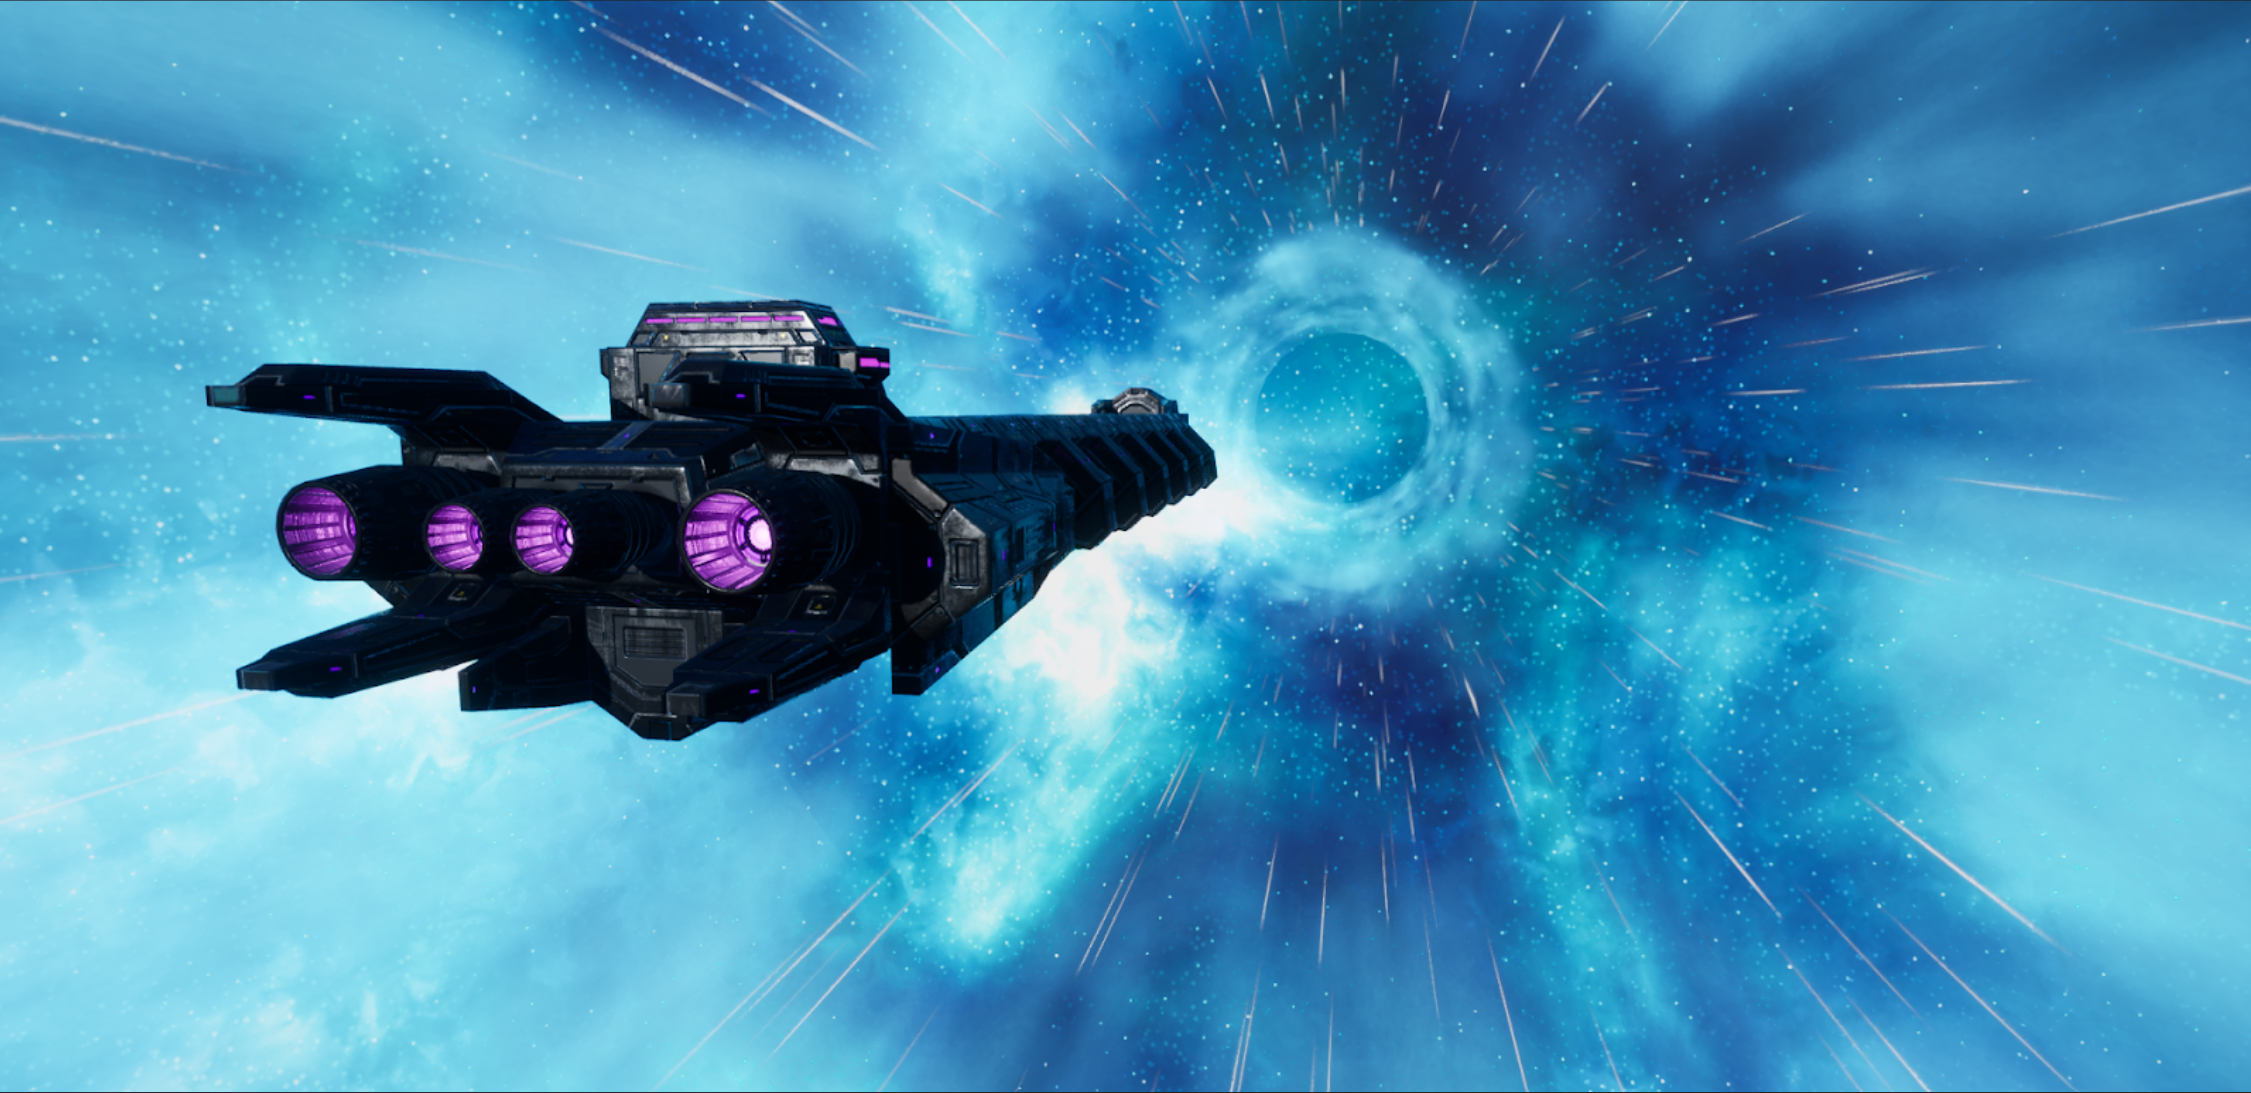
\includegraphics[width=6.0in]{aaafiles/teaser.png}
  \caption{Spaceship jumping into hyperspace. }
\end{teaserfigure}

% Processes all of the front-end information and starts the body of the work.
\maketitle

\section{Introduction}

For a long time, Unreal Engine 4 (UE4) uses the PhysX 3.3 physics engine \cite{physx} to drive its physical simulation calculations and perform all collision calculations. PhysX provides the ability to calculate accurate collision detection and simulate the physical interaction of objects in the scene. 
With the newly released Chaos Physics System \cite{ue4chaos}, developers are capable of achieving cinematic-quality visuals in real-time in scenes with massive-scale levels of destruction. Before Niagara Particle systems \cite{ue4Niagara}, the primary way to create and edit visual effects in UE4 was to use Cascade \cite{ue4cascade}. While both Cascade and Niagara can be used to make visual effects inside of Unreal Engine 4, Niagara became a complete replacement for Cascade, because Niagara is much more adaptable and flexible. 

The traditional workflow to make any massive destruction scenes relies heavily on the use of external third-party tools or plugins. However, Chaos allows developers to create and edit everything within the UE4 editor. We are interested in seeing how the Chaos physics system can be applied to traditional workflow, and we want to explore how Niagara can be integrated into the Chaos system. Therefore, we created a space-war scene that demonstrates the potential of the Chaos physics system.

We describe our contribution as follows:

\begin{itemize}
    \item We acquired and compiled UE 4.23 from the source code on multiple machines.
    \item We created some planets and space scenarios that exploit the features of Chaos physics in UE 4.23. 
    \item We explored methods to integrate Niagara particle effects with the Chaos workflow, such as triggering particle spawns upon Chaos Break Event. 
    \item We applied different property on different components of a single spaceship mesh.  
\end{itemize}

Moreover, we have released our project to the public at \url{www.github.com}.

% ---------------------------------------------------------------------
\section{Setup}

Since the Chaos Physics system is still currently under Beta, we need to obtain a source build version of the Unreal Engine in order to use this feature. In this section, we describe what we have done to obtain the required version of UE4. We consider this as a big achievement because compiling UE4 is not trivial, and we spent more than 10 hours in it, with most of the time spent on compiling the engine and the projects. 

\subsection{Source Code Acquisition}

Prerequisites:

\begin{itemize}
    \item Epic account
    \item GitHub account
    \item git or GitHub desktop
\end{itemize}

According to the official document from Epic, we first need to link our GitHub account to our Epic account; this step is trivial, but it requires an evaluation from Epic. Upon approval, our GitHub account will be added to Epic's Unreal Engine Organization on GitHub and will be granted access to its private repository for Unreal Engine. 

Fork the unreal engine repository and clone it to the local environment. Switch the branch to \textbf{Release} branch, which was initially Build 4.23.1. This step takes a while, but once it was finished, we will have complete access to UE4's source code on our local environment.

\subsection{Build and Compile}

Prerequisites:

\begin{itemize}
    \item Visual Studio 2015/2017/2019
\end{itemize}

\begin{figure}[ht]
  \centering
  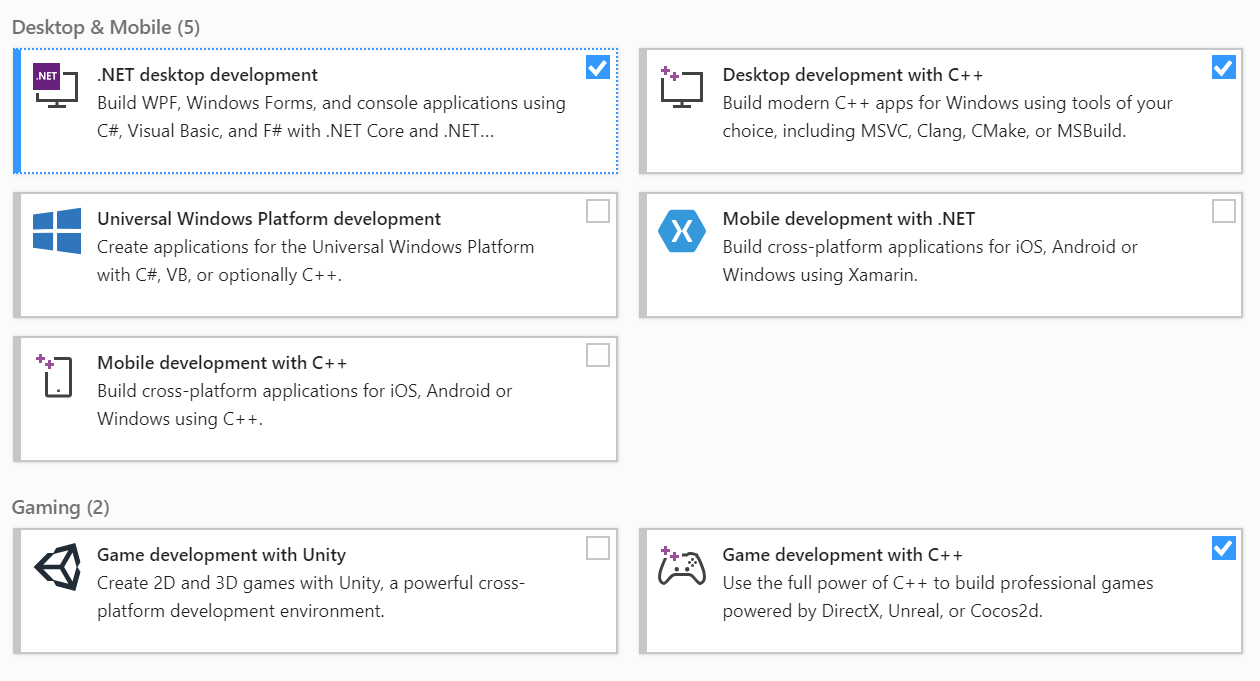
\includegraphics[width=\linewidth]{aaafiles/enviroment.png}
  \caption{Figure showing the correct configuration for Visual Studio Installer for this project Note that the .NET desktop development is essential to success. }
  \label{fig:visual_studio}
\end{figure}

\textbf{Install Environment:} Once the sourced code is obtained locally, and Visual Studio was correctly installed. Be sure to include C++ support as part of the install as indicated in Figure \ref{fig:visual_studio}, which is disabled by default. 

\begin{itemize}
    \item .NET desktop development
    \item Desktop development with C++
    \item Game development with C++
\end{itemize}

Due to the lack of documentation and tutorials on the internet, we have failed to compile the engine on the first try. After hours of diagnosis, we have determined the cause of failure was missing the a specific version of \textit{.NET framework}. 

Although \textit{.NET framework} was meant for C\# desktop development, a substantial amount of Unreal Engine's component were depending on this framework. Moreover, different component was depending on different version of the \textit{.NET framework}: installing only the latest version is not sufficient. 

\vspace{5mm}

\textbf{Build:} By default, Chaos features are turned off. To enable the use of Chaos. We first add the statement \textit{bCompileChaos = true;} into the \textbf{UE4Editor.Target.cs} file under the \textbf{Engine/Source} folder. 

In the 4.23 root folder, run the \textbf{Setup} batch file, then upon completion, run the \textbf{GenerateProjectFiles} batch file. This step takes the most of the time. The average total time on our desktop machines was approximately $4-5$ hours. These two batch file will download additional files to the machines, and after the process, another $~50 GB$ of storage is used. Do not try this at home. We did this on a School Lab Computer. 

\vspace{5mm}

\textbf{Compile:} In order to make the compilation process easier, we have installed additional Visual Studio Extension \textit{UnrealVS} provided by Epic. \textit{UnrealVS} provide various helper tools, such as the Batch Builder (figure \ref{fig:unrealvs}), to make the compile task simpler to use. 

\begin{figure}[ht]
  \centering
  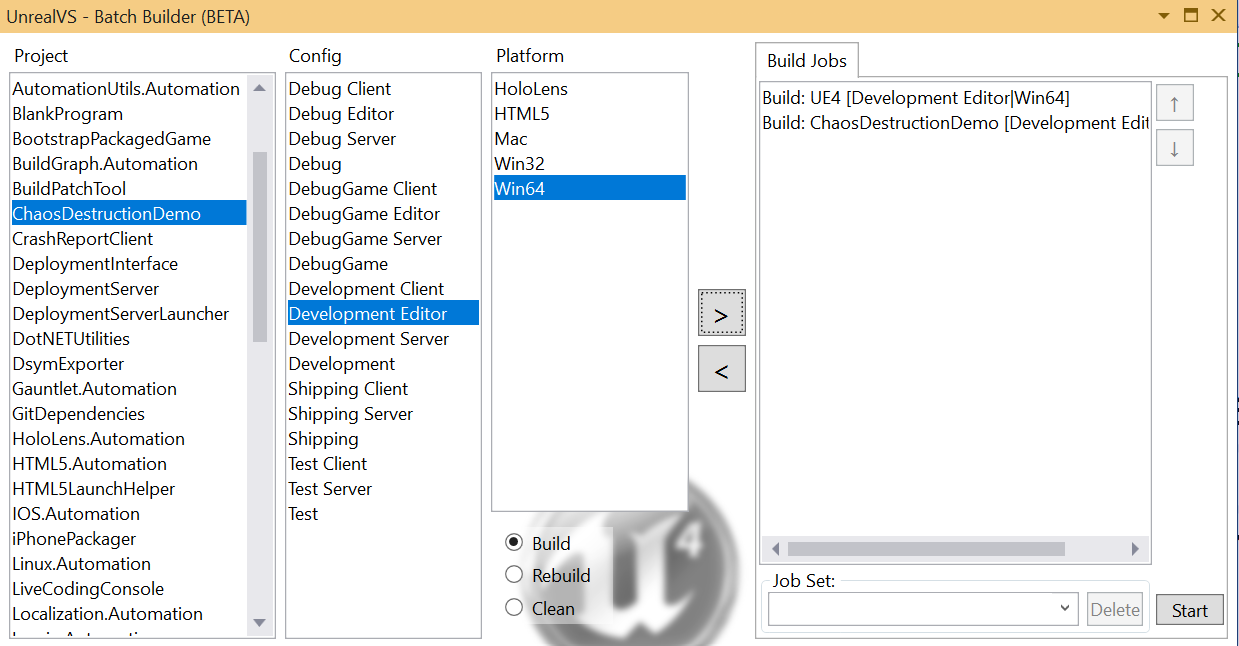
\includegraphics[width=\linewidth]{aaafiles/unrealvs.png}
  \caption{The correct Build Jobs used in this project. We first need to build the Development Editor of UE4 on Win64. Then build the Development Editor of ChaosDestructionDemo on Win64.}
  \label{fig:unrealvs}
\end{figure}

Following figure \ref{fig:unrealvs}, we can start compile binary executable of Unreal Engine as well as the Chaos Demo project. This process takes another $2-3$ hours, as a result, additional $60 GB$ of Binary and Intermediate files was generated. 

\subsection{Create project with Source Build}

At this stage, we have successfully compiled Unreal Engine 4.23.1 on our own environment. We can now start the Chaos Demo Project using this source build version of UE4, simply by double clicking the \textit{.uproject} files. 

% ---------------------------------------------------------------------
\section{Chaos Physics}

In this section, we are going to give an overview of the Chaos Physics System. However, we will not go over every detail of this system. We will only highlight the parts that are most used in our project. 

\subsection{New Features}

\begin{itemize}
    \item Chaos Editor
    \item Chaos Solver
    \item Chaos Niagara
    \item Planar Cut
    \item Editable Mesh
    \item Geometry
    \item Geometry Cache
    \item Field System
\end{itemize}

\begin{figure}
\begin{multicols}{2}
    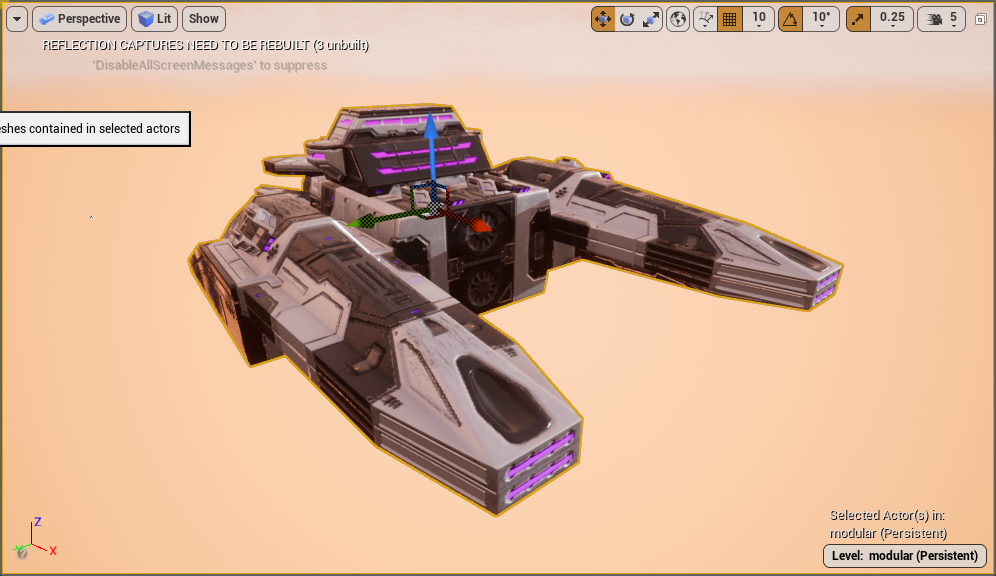
\includegraphics[width=\linewidth]{aaafiles/0.png}\par 
    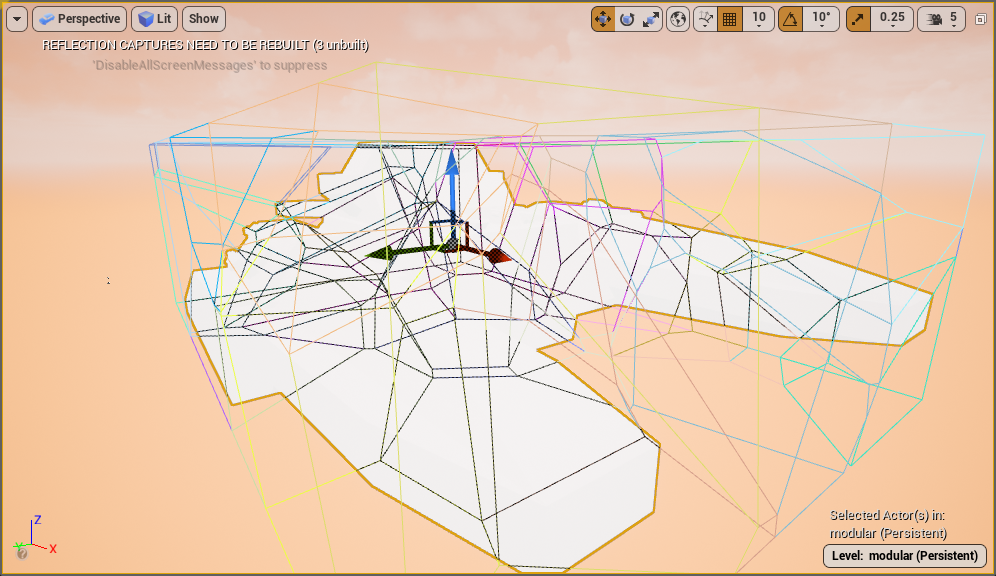
\includegraphics[width=\linewidth]{aaafiles/1.png}\par 
    \end{multicols}
\begin{multicols}{2}
    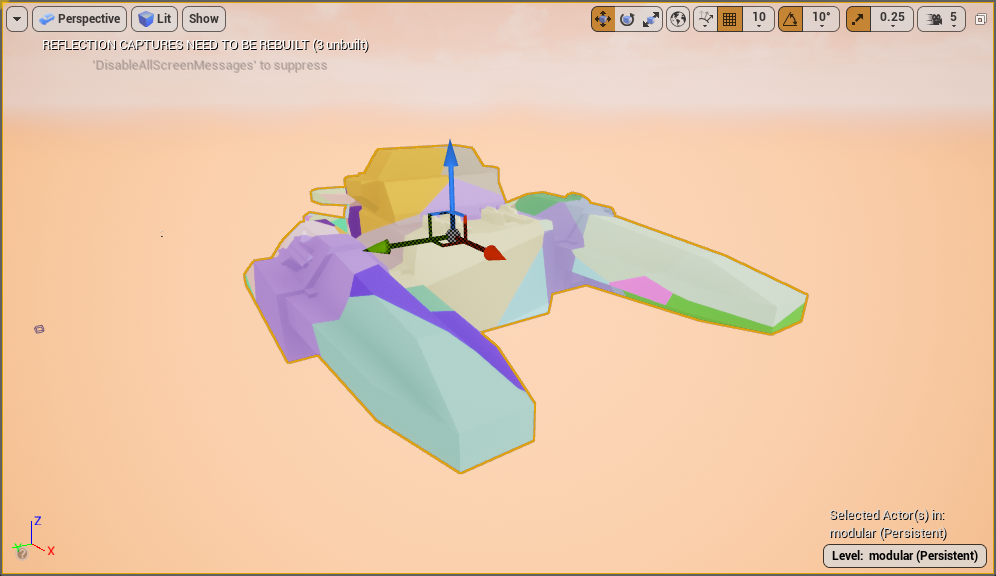
\includegraphics[width=\linewidth]{aaafiles/2.png}\par
    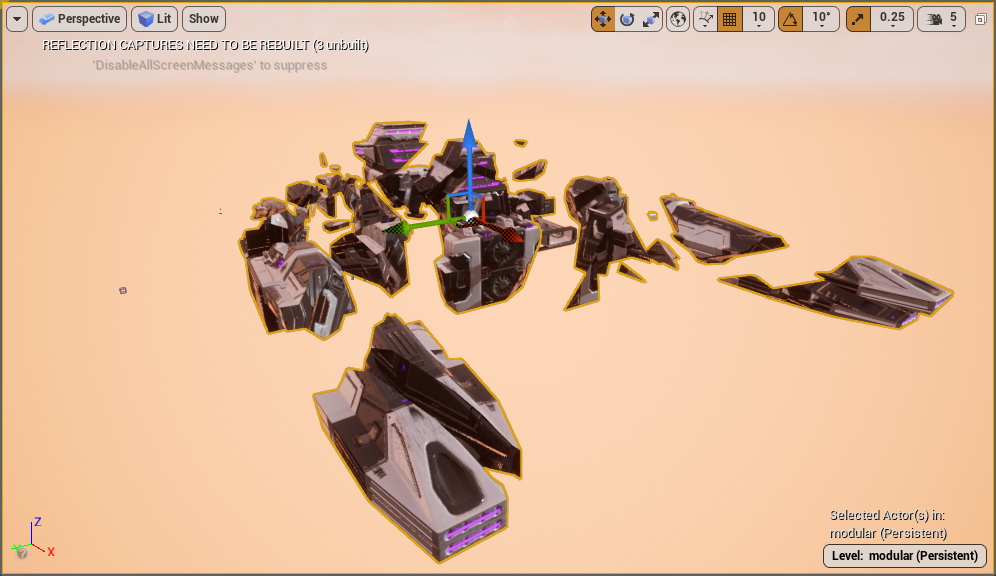
\includegraphics[width=\linewidth]{aaafiles/3.png}\par
\end{multicols}
\caption{Example of a mesh being transformed into a geometry collection.}
\end{figure}

\subsection{Geometry Collections}

Geometry collections is a new type of asset that allows the engine to break a mesh apart using the fracture editor. The process of creating geometry collections is very simple. With a couple of clicks, you can turn any mesh or groups of meshes into geometry collections.

\begin{figure}[ht]
  \centering
  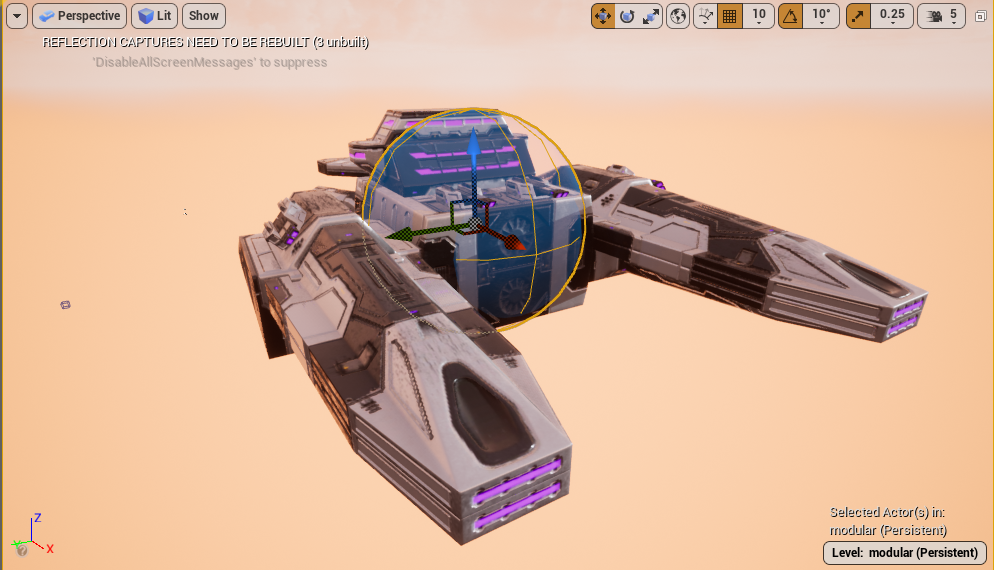
\includegraphics[width=\linewidth]{aaafiles/force.png}
  \caption{Figure shows a visual representation of the volume occupied by a force field.}
  \label{fig:force}
\end{figure}

\begin{figure*}
\begin{subfigure}{.5\textwidth}
  \centering
  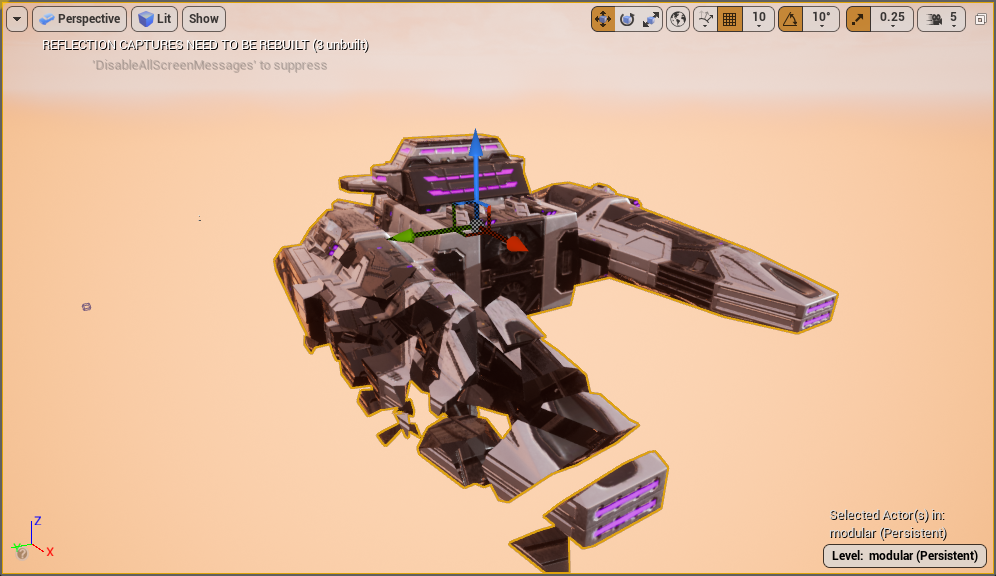
\includegraphics[width=.9\linewidth]{aaafiles/4.png}
  \caption{}
\end{subfigure}%
\begin{subfigure}{.5\textwidth}
  \centering
  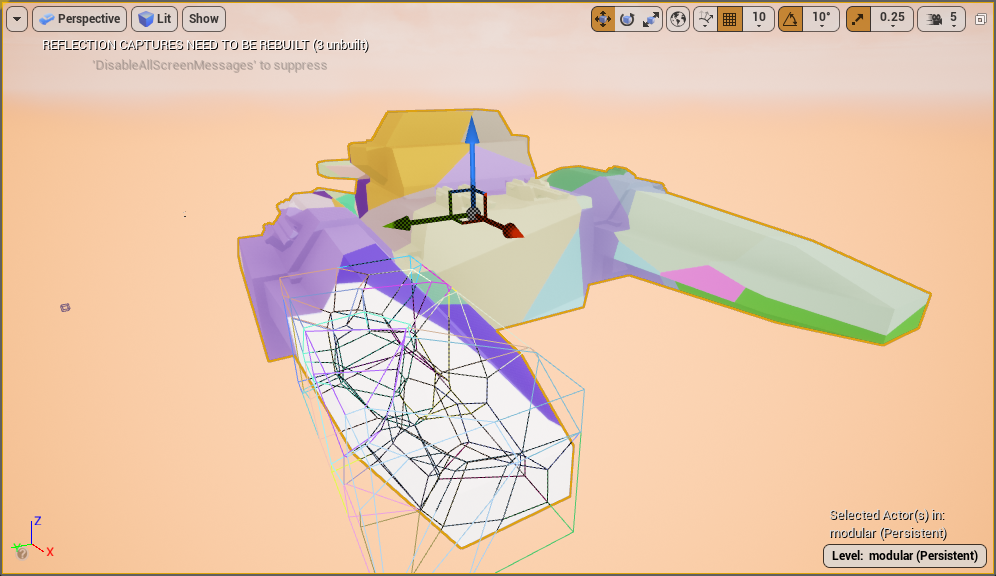
\includegraphics[width=.9\linewidth]{aaafiles/5.png}
  \caption{}
\end{subfigure}
\caption{(a) Normal view of breaking a smaller piece of a geometry collection. (b) Clustering view of a sub-level fracturing. Note only the right wing of the spaceship is fractured. We demonstrate that we can hierarchically fracture geometry collection in Chaos. }
\label{fig:fig}
\end{figure*}

\begin{figure*}
\begin{subfigure}{.5\textwidth}
  \centering
  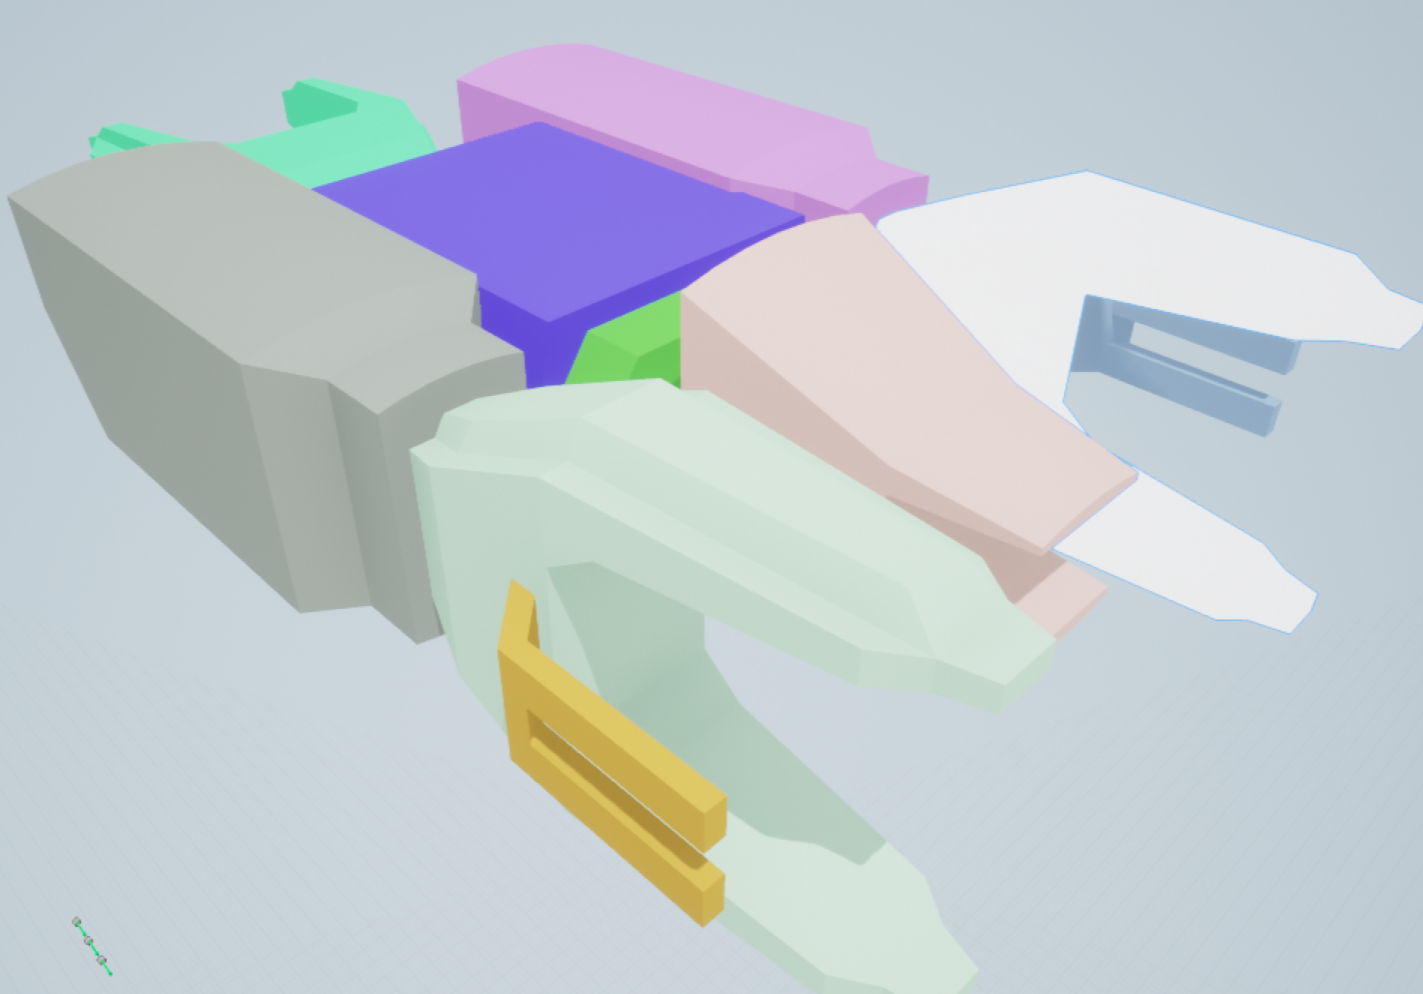
\includegraphics[width=.9\linewidth]{aaafiles/decomposition.png}
  \caption{}
\end{subfigure}%
\begin{subfigure}{.5\textwidth}
  \centering
  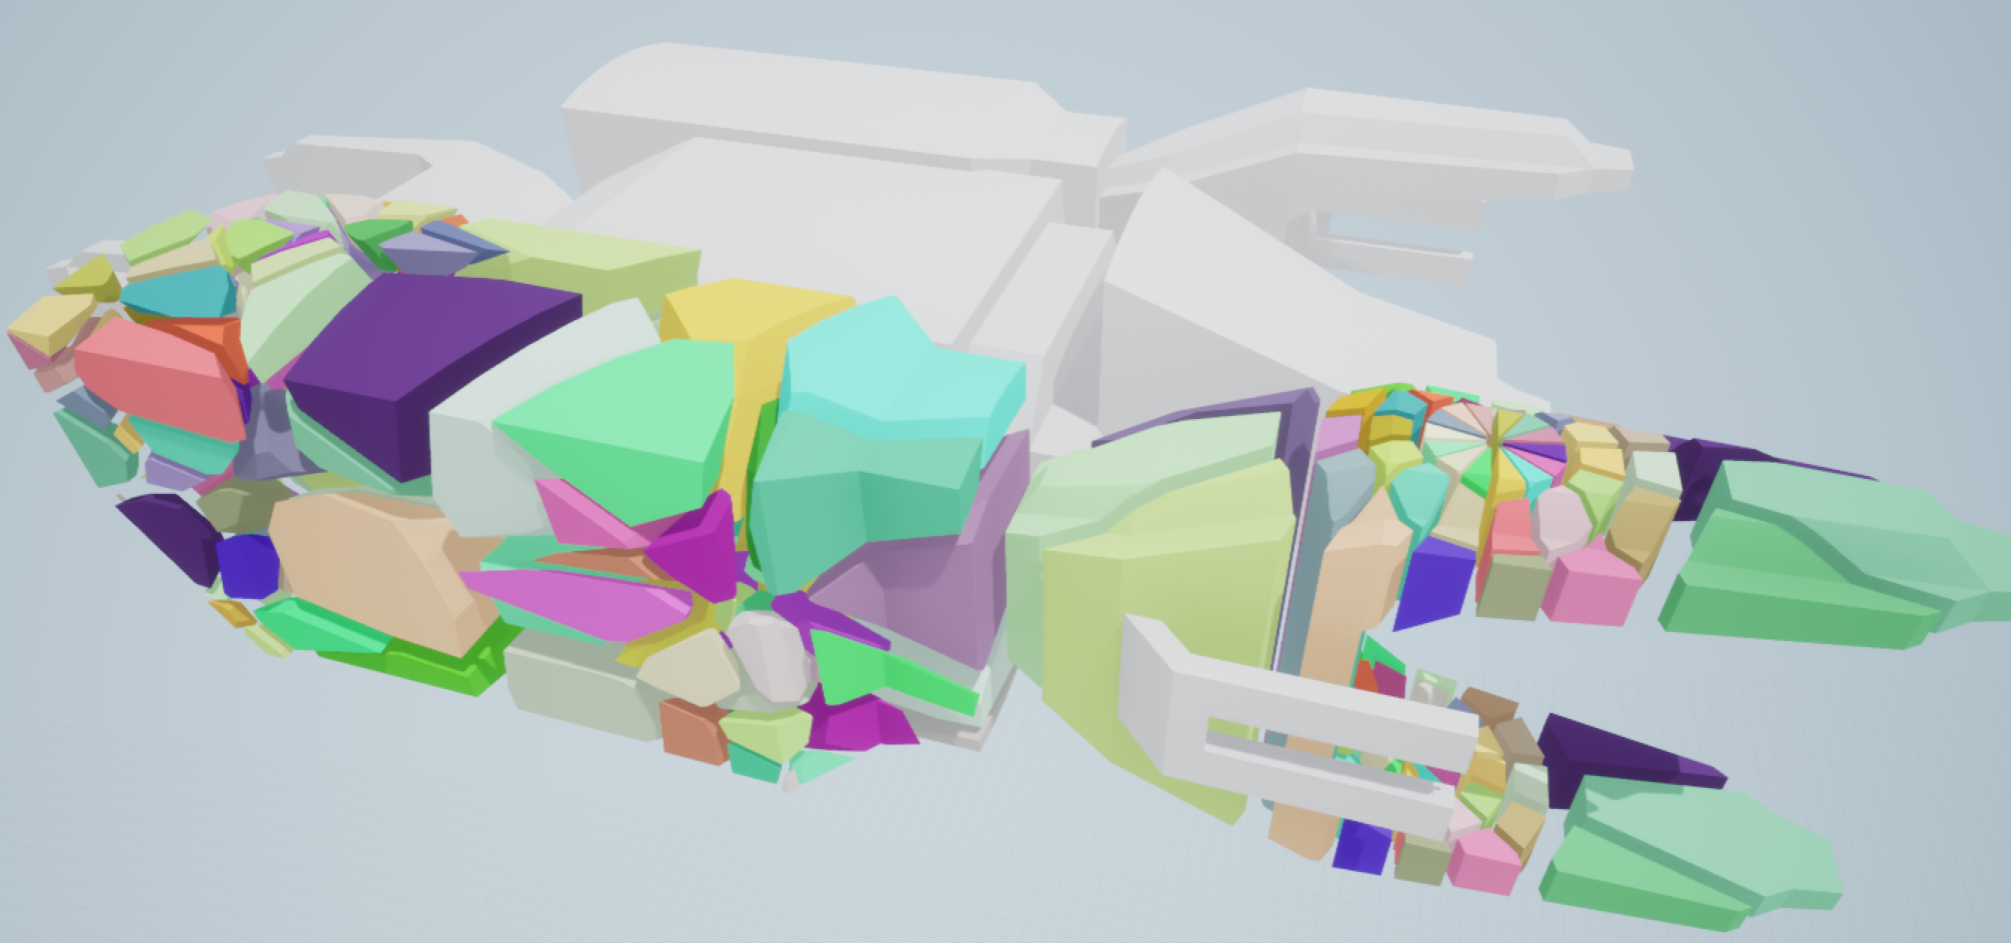
\includegraphics[width=.9\linewidth]{aaafiles/dec2.png}
  \caption{}
\end{subfigure}
\caption{(a) Decomposed spaceship mashes. (b) Example of showing different fracturing properties being applied to different parts of the ship. Note this is different from Figure \ref{fig:fig}, we have manually partitioned the original static mesh into pieces. This approach gives artist more control to produce desired visual effects. }
\label{fig:decomposition}
\end{figure*}

\subsection{Fracturing and Clustering}

In the fracture editor, click the generate geometry collection button under the select tab, adjust the settings until you are satisfied with the results, and then select fracture to finish creating your geometry collection. This process can be used in single or multiple meshes, including the ones inside blueprints.

Clustering is the process on which several meshes are fracture together, or when a smaller piece of an already existing geometry collection is fractured. A geometry collection can have several clusters (Figure \ref{fig:fig}), and each cluster can have a different strain force required for it to break apart. 

\subsection{Anchor Fields}

Anchor fields are a special type of field because their logic works differently than most of the others. Its purpose is to hold portions of a geometry collection in place while the rest breaks. They must be established in the construction state so that a connection graph is made before the simulation runs. Therefore, the anchor fields must be initialized in the "initialization fields" tab of the geometry collection on which it will be used.

Anchored geometry will remain established until a strained is placed upon it. However, during our tests, we also found out that if the geometry collection is too big, you will need either a bigger anchor field or multiple anchor fields, to hold the structure in place.

\subsection{Fields}

Fields are a way to directly affect the physics simulation in a given volume, and are used to produce different behaviors or brake effects.

\subsection{Field Types}

\begin{itemize}
    \item Cluster Strain
    \item Force
    \item Angular Torque
    \item Noise and Culling
    \item Sleep and Disable
    \item Internal Strain
\end{itemize}

\subsection{Used Fields}

Although there are many types of force fields, we decided to make use of a simple force field (figure \ref{fig:force}). These force fields apply a specified amount of force and strain to geometry collections within a given volume. Its basic function is first to apply enough strain to break a geometry collection, and then apply a force with which it will push away the broken pieces of the structure. Moreover, we also made use of anchor fields in order to keep our meshes in place.

% ---------------------------------------------------------------------
\section{Niagara Particle system}

Unreal Engine 4's Niagara visual effects system are used for creating and previewing particle effects in real time. 

\subsection{Overview}

Niagara particle systems have been broken up into the following two parts:

\textbf{Niagara Emitter} This is a single visual effect that will be combined with other Niagara Emitters to make a Niagara System. For example, in making explosion effects for our project, we have multiple emitters represents fire, smokes, and embers particles. 

\textbf{Niagara System} This contains everything needed to make up a single effect. Continuing with our example, this would be the completed explosion effect that contains the Niagara Emitters for the smoke, fire, distortion, and embers. 

\subsection{Chaos Integration}

However, while Niagara sounds promising, the way that Niagara works in Chaos Projects is slightly different. 

\textbf{Chaos Data Interface}: The most important thing to note is the Chaos Data, this is an abstract interface class. A Niagara system must implements the Chaos Data Interface, and will be active for all rigid bodies driven by the world Chaos Solver. Inside the Niagara Effects system, events listed below are listened for through the Chaos Data Interface. 


\begin{figure}[ht]
  \centering
  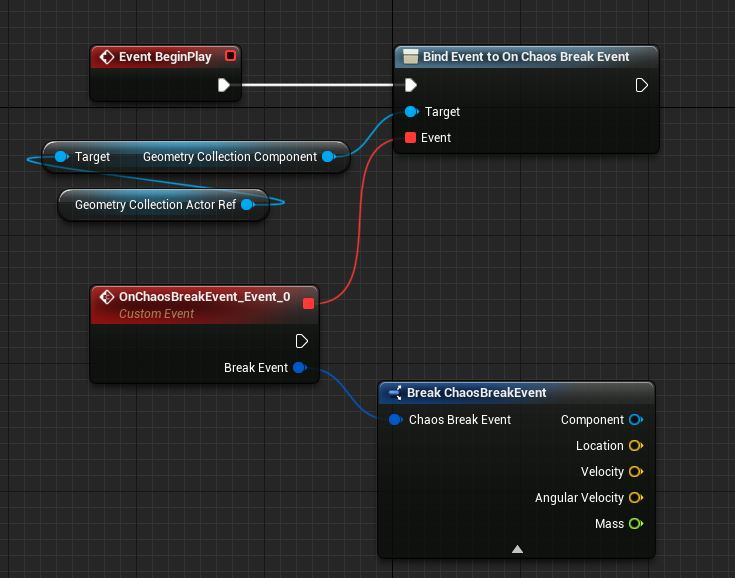
\includegraphics[width=\linewidth]{aaafiles/event_blueprint.png}
  \caption{Blueprints in our project, showing how we can bind the Chaos break event of a Geometry Collection Actor to an custom Event. }
  \label{fig:chaos_event}
\end{figure}

\textbf{Events:} There are three types of events in Chaos, listed below,

\begin{itemize}
    \item Break Event
    \item Collision Event
    \item Trail Event
\end{itemize}

Geometry Collections can send collision and break events that can be used to trigger gameplay. In our project, we are sending events to trigger the Niagara Particles to spawn the particles (Figure \ref{fig:chaos_event}). For the Geometry Collection to send these events, the Notify Collisions (for collision events) or Notify Breaks (for break events) must be enabled on the Geometry Collection Actor. 

As shown in Figure \ref{fig:chaos_event}, we can bind any types of Chaos Events to a CustomEvent (named \textit{OnChaosBreakEvent\_Event\_0}). Thus, when Chaos event is triggered, we can receive the information such as the following:

\begin{itemize}
    \item Component: Component
    \item Location: FVector
    \item Velocity: FVector
    \item Angular Velocity: FVector
    \item Mass: float
\end{itemize}

With this information, we can make things like spawn a Niagara System Actor at \textit{Location}, giving it some initial speed properties \textit{Velocity} and more. 

\textbf{Chaos Solvers:} It is vital to understand where the Chaos events are stored. By default, Chaos automatically creates a \textit{Chaos World Solver} actor to manage Chaos related computation. It is an actor that will be placed on the Map. Chaos solvers within the Chaos Destruction system can store a list of the collision, breaking, and trailing events as the simulation runs. Inside the Niagara Effects system, those events are listened for through the Chaos Data Interface. 

% ---------------------------------------------------------------------
\section{Results}

We describe our setup of our scene and present the results in this section. 

\subsection{Our scene}

\begin{figure}[ht]
  \centering
  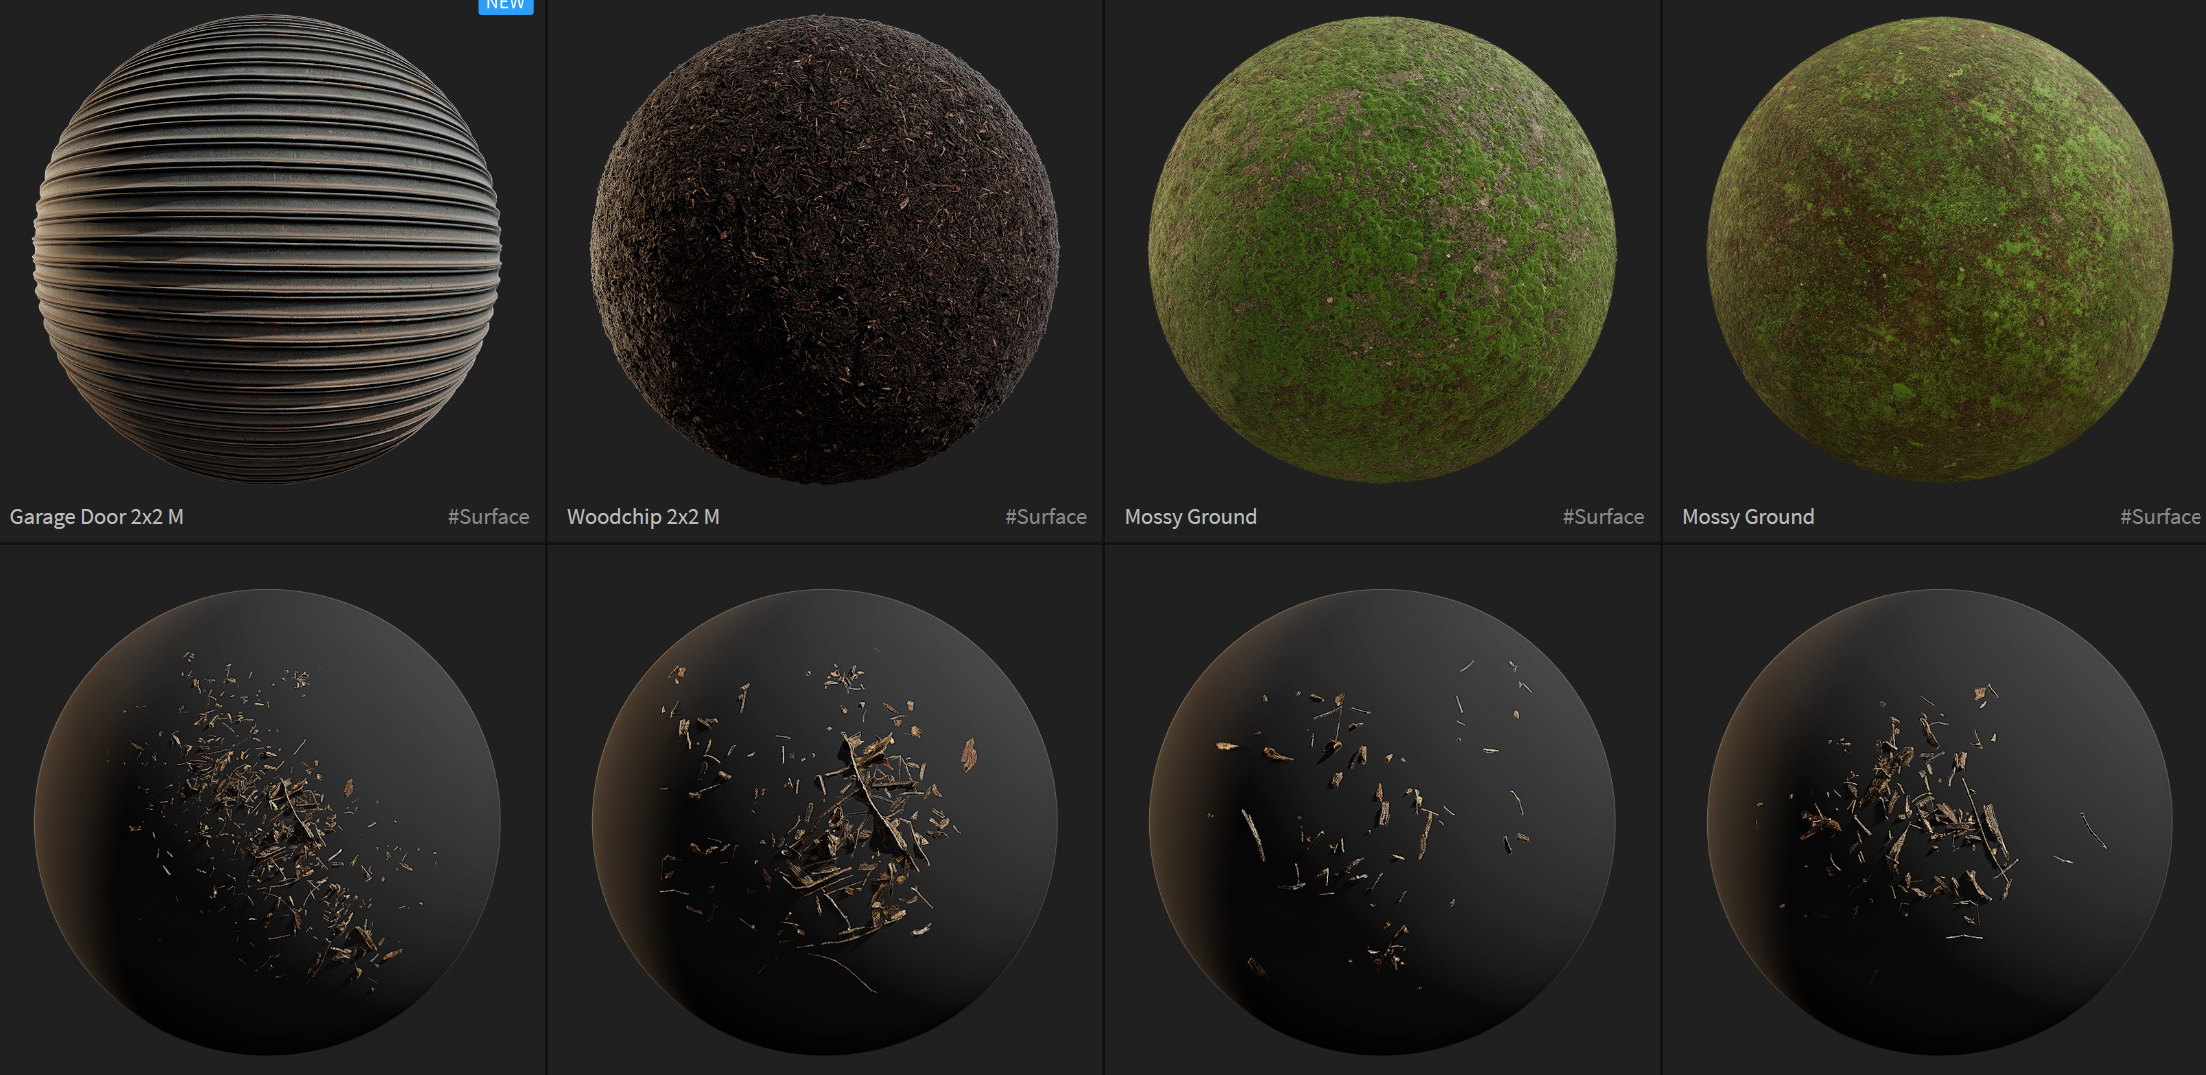
\includegraphics[width=\linewidth]{aaafiles/quixel.png}
  \caption{Megascans is a massive online scan library of high-resolution, consistent PBR calibrated surface, vegetation and 3D scans, also including desktop applications for managing, mixing and exporting your downloaded scan data.}
  \label{fig:quixel}
\end{figure}

We first created a Skybox Blueprint actor, using space textures from online assets store. The Skybox actor is internally represented as a sphere static mesh. 

We created an over planet landscape with the Unreal terrain tools. We initially wanted to use the newly released terrain tools from 4.24. However, Chaos system is still not integrated into the Engine yet, and we were not able to compile it from source again. Thus we simply decided to use the traditional terrain editor. We imported textures from Quixel Megascans \cite{quixel}, which recently announced to join force with Epic. 

We decomposed the static mesh asset of a spaceship obtained from assets store into multiple parts. The purpose of breaking the one single static mesh is to manually set different properties to different pieces of the spaceship. This step allows the Chaos physics engine to break the spaceship in a more realistic way; as a result, our experimental parameters presents a good final visual result. Table \ref{table:setting} shows a detailed setting of our decomposed ship.

\begin{table}[]
\begin{tabular}{|c|c|c|c|c|c|c|}
\hline
       & sm1 & sm2  & sm3 & sm4 & sm5 & sm6 \\ \hline
type   & U   & R    & U   & U   & U   & P   \\ \hline
radius & -   & 50.0 & -   & -   & -   & -   \\ \hline
min    & 20  & -    & 15  & 10  & 5   & -   \\ \hline
max    & 20  & -    & 25  & 30  & 35  & -   \\ \hline
cuts   & -   & -    & -   & -   & -   & 3   \\ \hline
\end{tabular}
\caption{Settings of our composited spaceship. This setting turned out to have the best visual effect.}
\label{table:setting}
\end{table}

Our demo space scene can run on Win64 Desktop with a frame rate of 60 fps, see Figure \ref{fig:result}. Refers to Figure \ref{fig:new_result} and Figure \ref{fig:new_result2} for updates.

% ---------------------------------------------------------------------
\section{Conclusions and Future Work}


\begin{figure*}
\begin{subfigure}{.5\textwidth}
  \centering
  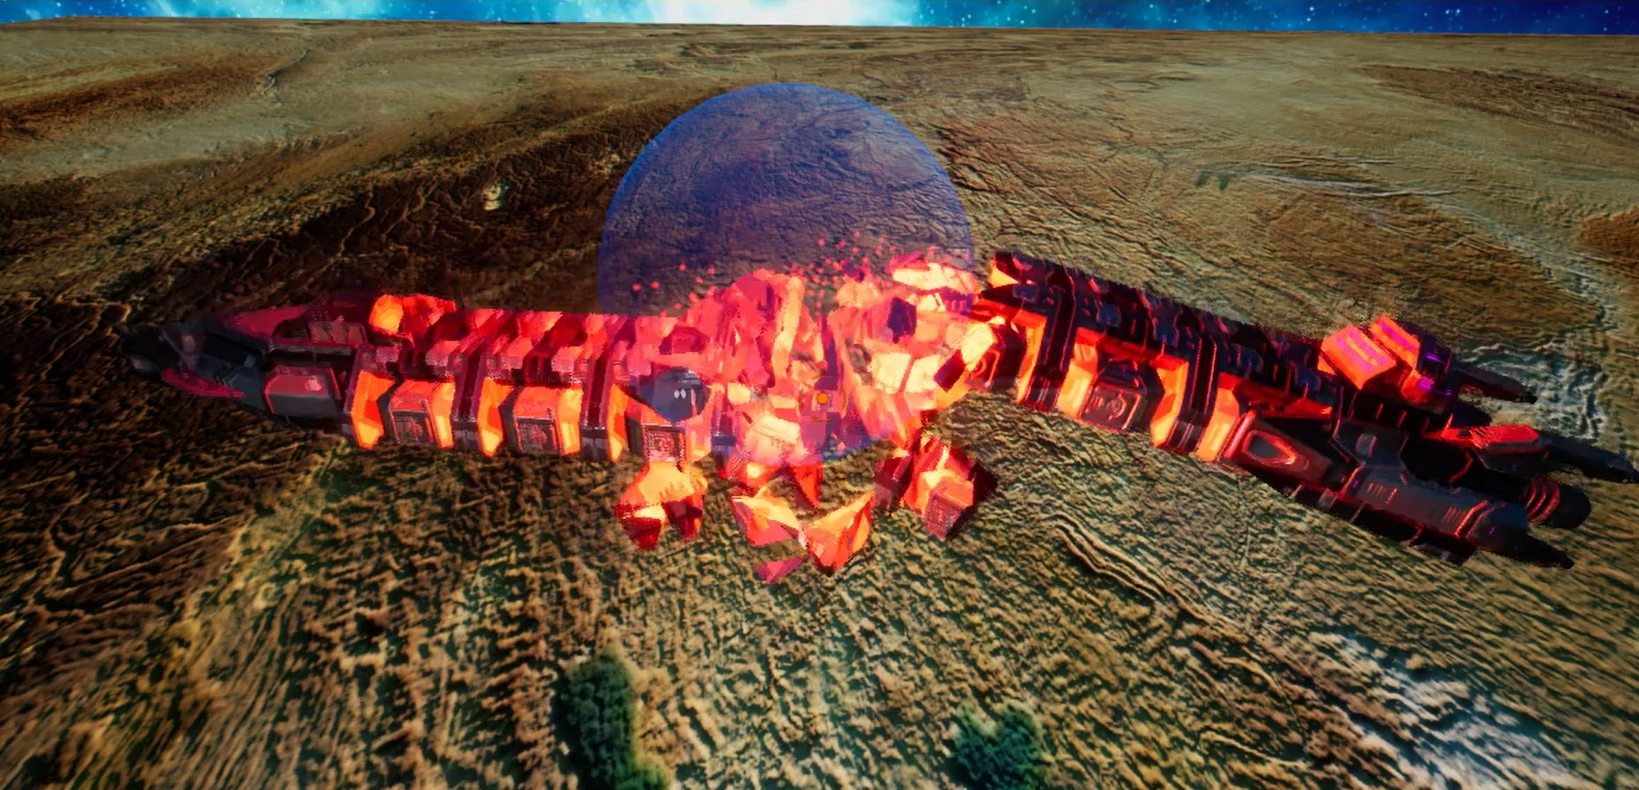
\includegraphics[width=\linewidth]{aaafiles/result1.png}
  \caption{}
\end{subfigure}%
\begin{subfigure}{.5\textwidth}
  \centering
  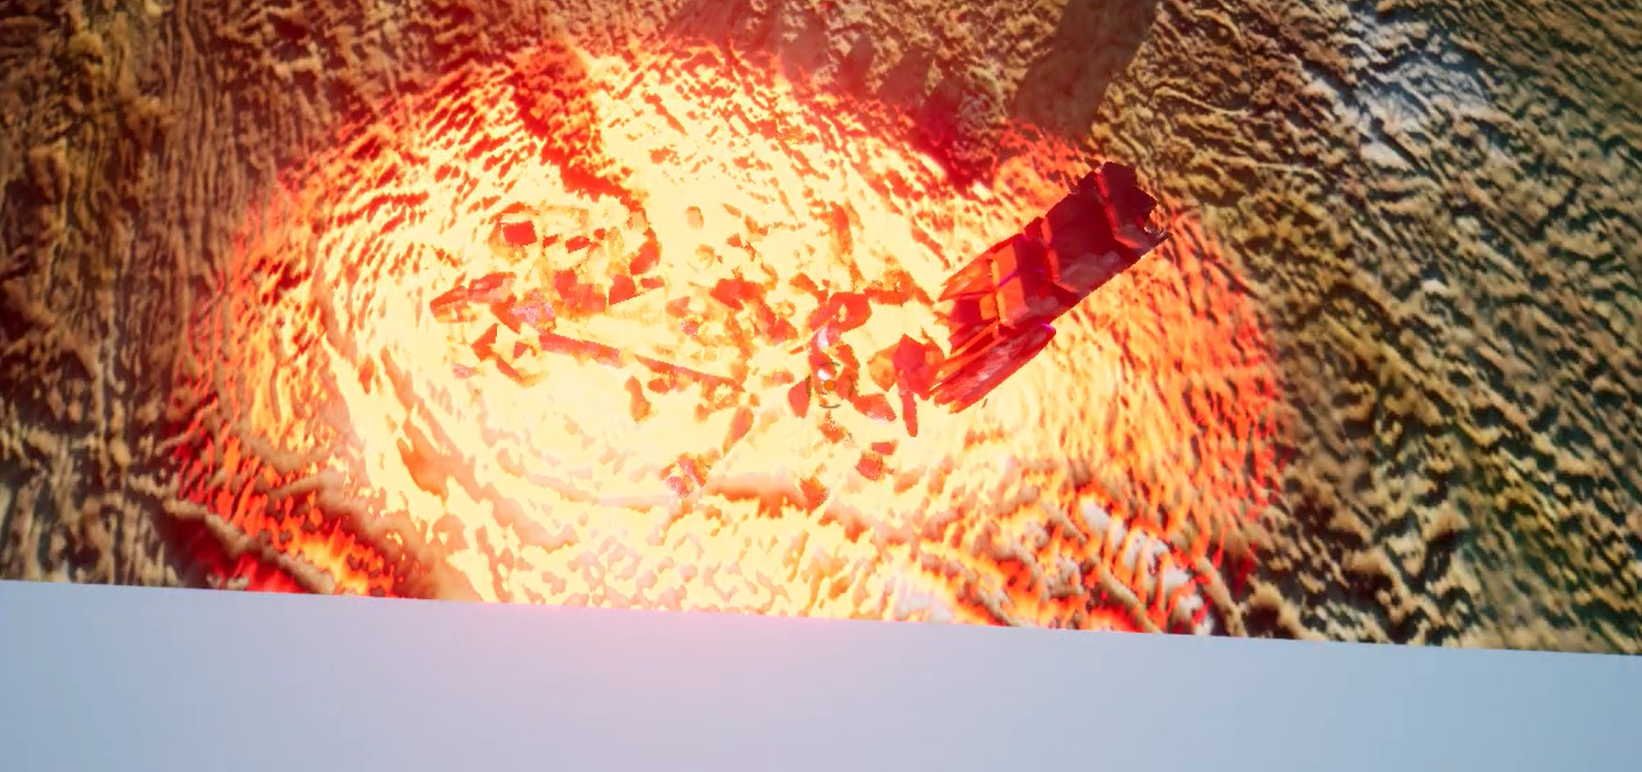
\includegraphics[width=\linewidth]{aaafiles/result2.png}
  \caption{}
\end{subfigure}
\caption{(a) Chaos destruction event happening at timestamp $t_0$, the spaceship is exploding. (b) After the first explosion happens, parts of the spaceship crush on the ground at time $t_1$. This has triggered a Collision event, and illuminating particles spawned.}
\label{fig:result}
\end{figure*}

\begin{figure*}
    \centering
    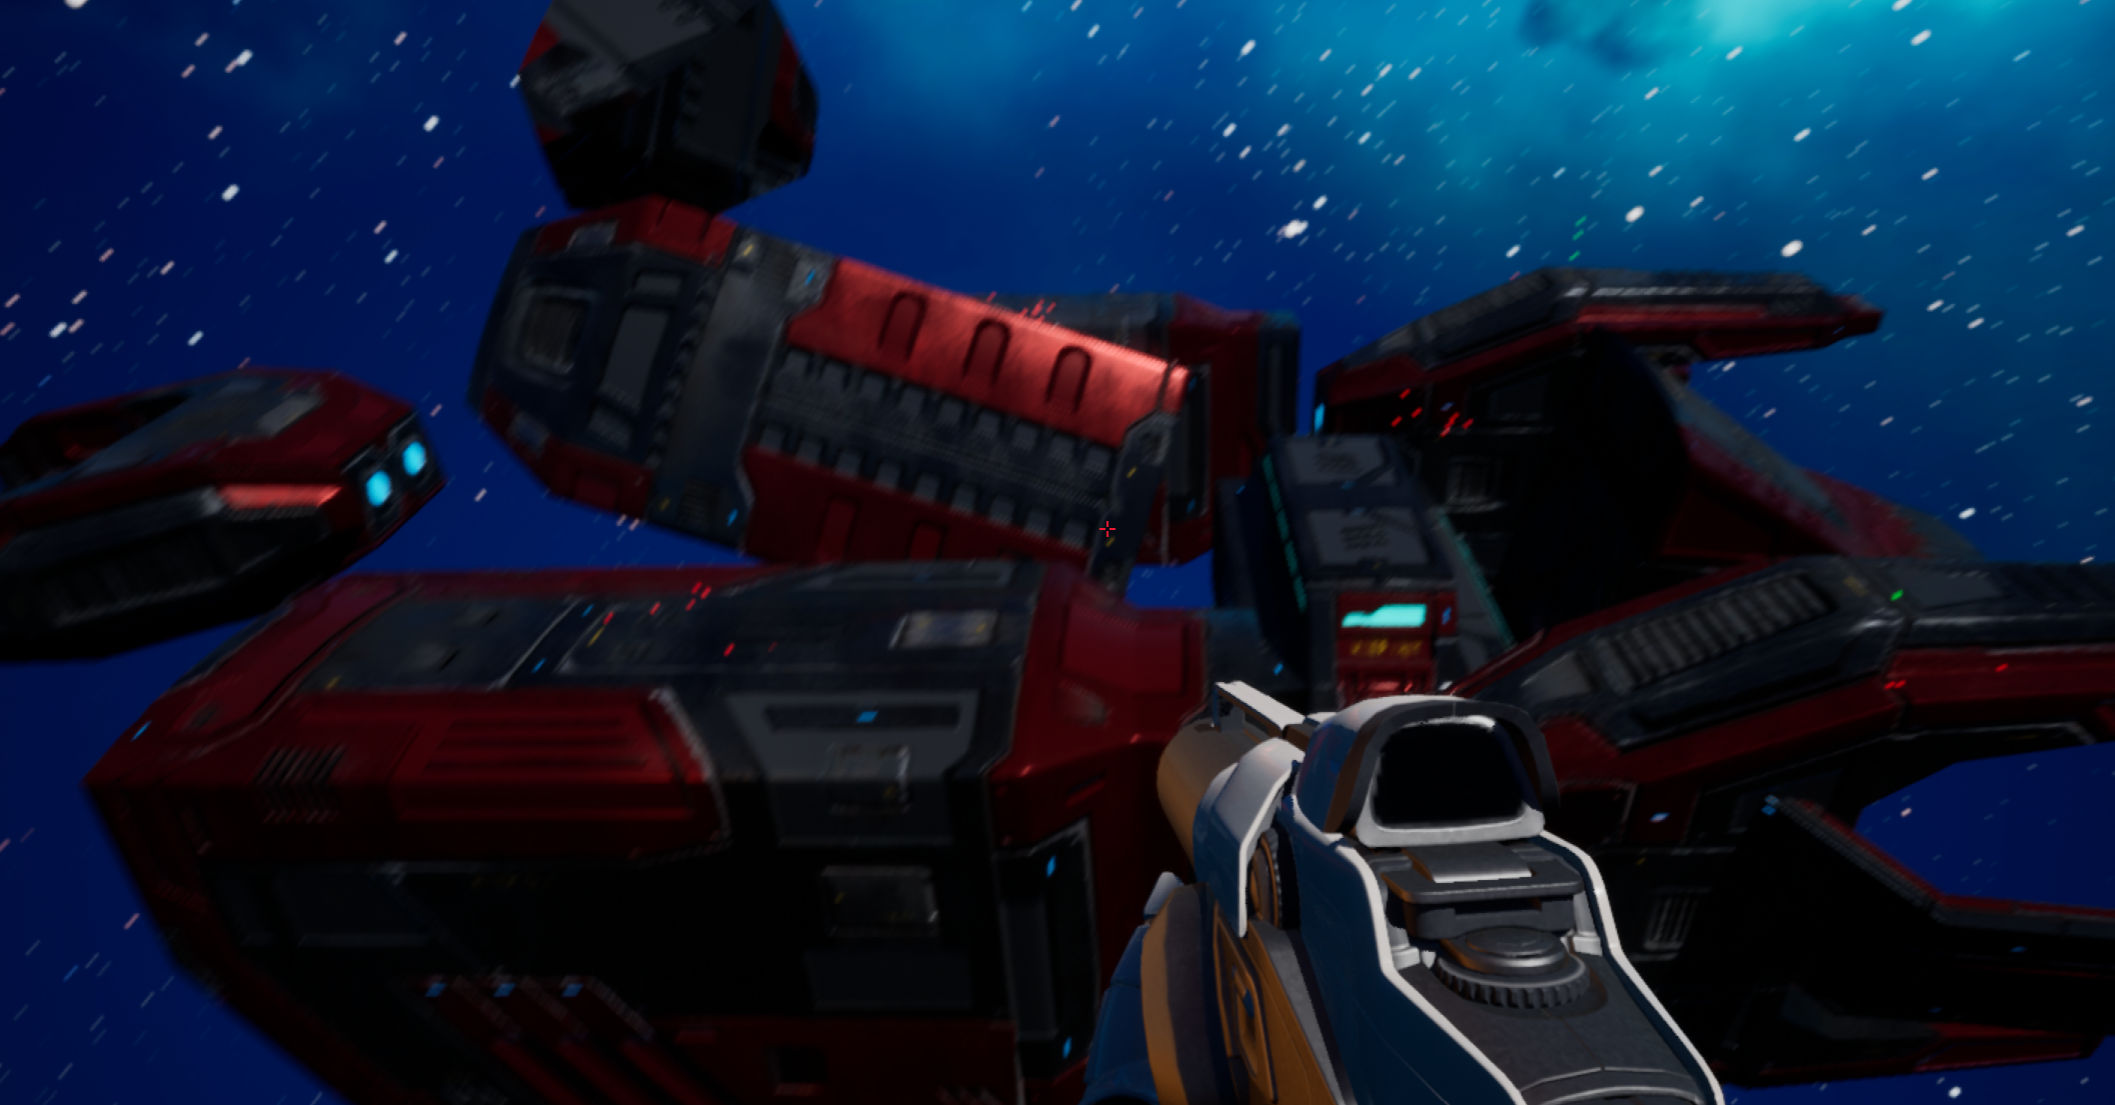
\includegraphics[width=.8\linewidth]{aaafiles/newresult.png}
    \caption{At timestamp $t_0$, a break even is triggered on a modified(decomposited) space mode. see Figure 2 \ref{fig:new_result2}}
    \label{fig:new_result}
\end{figure*}

\begin{figure*}
    \centering
    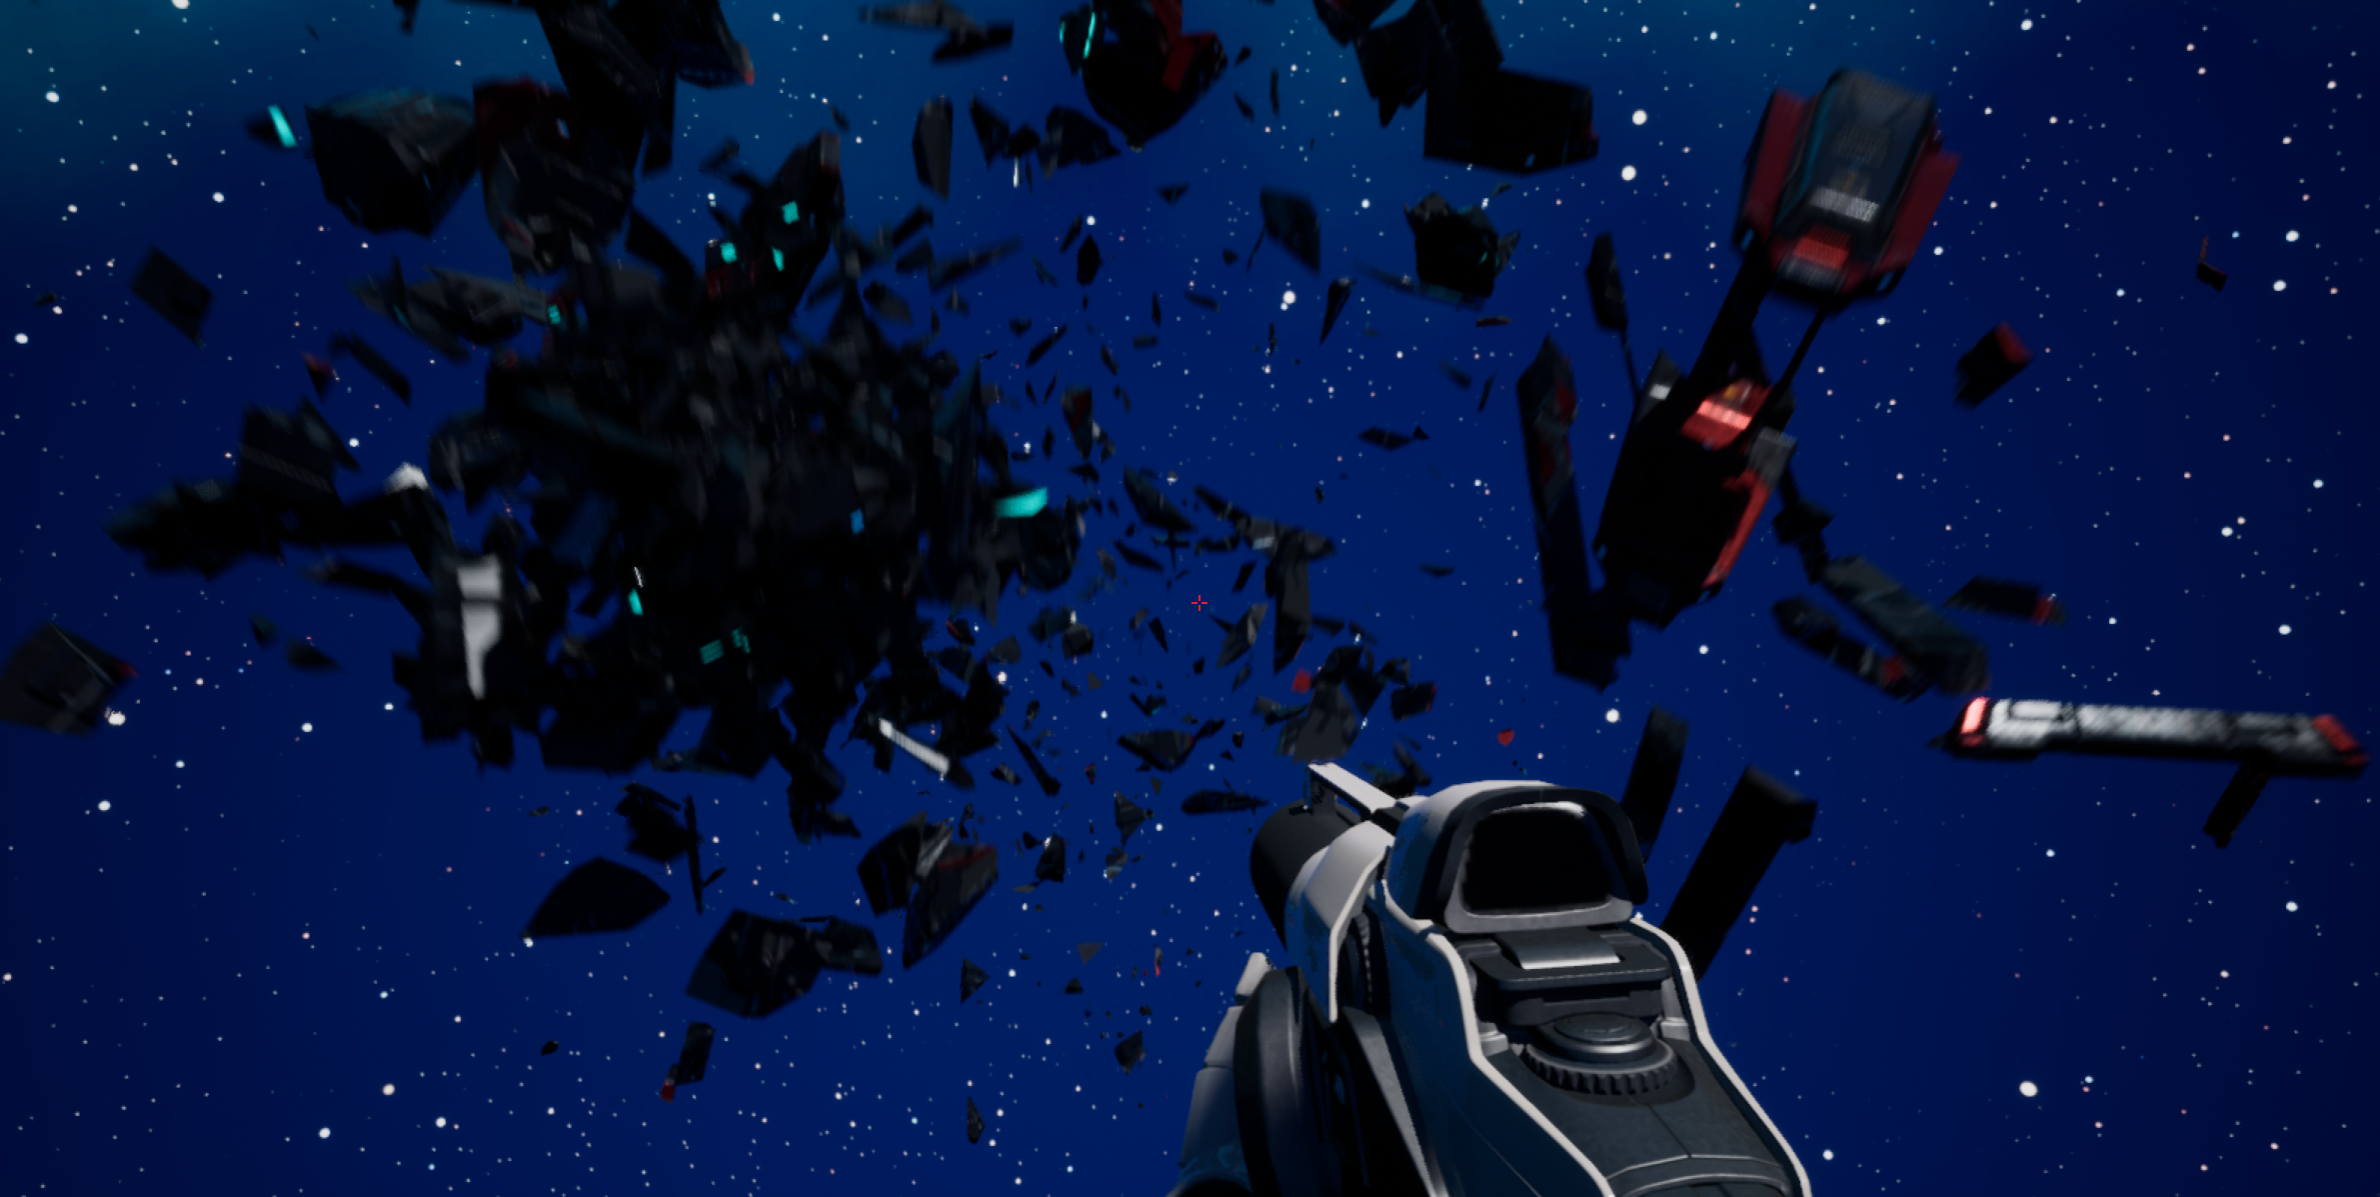
\includegraphics[width=.8\linewidth]{aaafiles/newresult2.png}
    \caption{The most important figure, this figure shows the visual result of destructing a spaceship with setting from Table \ref{table:setting}. As shown in the figure, part of the spaceship is broken into smaller pieces, where are others are larger and grouped together. This is because we have manually applied different material properties on different parts of the ship. }
    \label{fig:new_result2}
\end{figure*}

In summary, we have successfully compiled UE 4.23 from the source code on multiple machines. We have successfully created an over planet space scenarios that exploit the features of Chaos physics. Most significantly, we proposed multiple methods to integrate Niagara particle effects with the Chaos workflow. Equally significant, we have successfully set up the different levels (materials) on the spaceship as promised.

After conducting this research and tried out Chaos, we see that Epic has ambitious plans to replace its original PhysX 3.3 physics engine with Chaos gradually. At the same time, Epic is also considering to substitute Cascade with Niagara completely. 

Due to inexperience in UE4 and the shortage of time, we were incapable of creating the initially proposed plan: build an interactive star-war like an arcade shooting game. For future works, we are interested in seeing the following: 

\begin{itemize}
    \item Manipulating Gravity. 
    \item Caching in Chaos.
    \item Interactive arcade shooting game with many spaceships. 
\end{itemize}

Finally, the latest stable release of Unreal Engine 4.24 came out on December 9, 2019; a lot of new features added, such as the new Landscape tool. According to the development blog, and commit history, a few changes to the Niagara Particle system has been made. Although Chaos Physics System is still not integrated into the release version yet, we believe that once it completes its Beta test and is added to the Engine, Unreal Engine 4 will become the most powerful tool to create massive destruction. 



\begin{acks}
The authors would like to thank Montana Fowler for providing excellent lab tutorials on Niagara Particle systems. These tutorials made our project much easier to work with. The authors would also like to thank Professor Angus Forbes for providing valuable feedback on our work during office hours and class presentations. 
\end{acks}

\bibliographystyle{ACM-Reference-Format}
\bibliography{aaatemplate}
\end{document}